\documentclass[10pt]{beamer}

\usepackage{xeCJK}
\setCJKmainfont{Noto Sans CJK SC}
\xeCJKsetup{PunctStyle=kaiming,CJKspace=true,CheckSingle=true} 

\usepackage{subfigure}
\usepackage{amssymb, amsmath, amsfonts,verbatim}
\usepackage{tikz}
\graphicspath{ {./} }
\usetikzlibrary{matrix,arrows,fit,backgrounds,mindmap,plotmarks,decorations.pathreplacing}

\usepackage{pgfplots}
\pgfplotsset{compat=1.12}
\pgfdeclarelayer{background}
\pgfsetlayers{background,main}

\tikzset{decoration={name=none},}

\newlength\figureheight
\newlength\figurewidth

\newcommand{\tikzdir}[1]{#1.tikz}
\newcommand{\inputtikz}[1]{\input{\tikzdir{#1}}}

\newcommand{\tI}{\tilde {\mathcal I}}
\newcommand{\tA}{\tilde A}
\newcommand{\ty}{\tilde y}
\newcommand{\tx}{\tilde x}
\newcommand{\tw}{\tilde w}
\newcommand{\tv}{\tilde v}
\newcommand{\tC}{\tilde C}
\newcommand{\tP}{\tilde P}
\newcommand{\Ic}{{\mathcal I^c}}
\newcommand{\J}{{\mathcal J}}
\newcommand{\K}{{\mathcal K}}

\DeclareMathOperator{\Smin}{Smin}
\DeclareMathOperator{\Smid}{Smid}
\DeclareMathOperator{\Smax}{Smax}
\DeclareMathOperator{\MSE}{MSE}
\DeclareMathOperator{\rank}{rank}
\DeclareMathOperator{\Med}{Med}
\DeclareMathOperator{\Max}{Max}
\DeclareMathOperator{\Min}{Min}
\DeclareMathOperator{\tr}{tr}
\DeclareMathOperator{\Cov}{Cov}
\DeclareMathOperator{\logdet}{log\;det}
\DeclareMathOperator{\argmin}{arg\;min}
\DeclareMathOperator{\argmax}{arg\;max}
\let\Tiny\tiny

\title[Secure CPS]{Security of Cyber-Physical Systems}
\author[Yilin Mo]{Yilin Mo}
\institute[Tsinghua]{
  Department of Automation\\ Tsinghua University\\
}
\date[Nov 17, 2018]{ Nov 17th, 2018\\ 
  \small Joint Work with Bruno Sinopoli, Sean Weerakkody, Hanxiao Liu and Richard Murray}

\usetheme[subsectionpage=none,block=fill]{metropolis}
\definecolor{thupurple}{RGB}{102,8,116}
\definecolor{caltechcolor}{RGB}{102,8,116}
\setbeamercolor{title separator}{fg=black!50}
\setbeamercolor{frametitle}{bg=thupurple!70!black}
 

\begin{document}

\maketitle 

\section{Introduction}

\begin{frame}{个人简介}
  \begin{itemize}
  \item  2003-2007  清华大学自动化系,学士学位
  \item  2007-2012 Department of Electrical and Computer Engineering, Carnegie Mellon University, 博士学位, 论文题目:\,\textit{``Secure Detection, Estimation and Control of Cyber-Physical Systems''}
  \item  2013-2013 Department of Electrical and Computer Engineering, Carnegie Mellon University, 博士后
  \item  2013-2015 Department Computing+Mathematical Sciences, California Institute of Technology, 博士后
  \item  2015-2018 School of Electrical and Electronic Engineering, Nanyang Technological University, 助理教授
  \item 2017 获国家第14批青年千人
  \item 2018 现任清华大学自动化系副教授
  \end{itemize}
\end{frame}

\begin{frame}{Overview of My Research}
\begin{block}{Networked Control System}
  Understanding the interaction between control and communication.
 \begin{itemize}
  \item Kalman filtering with intermittent observation
  \item Sensor/Actuator Scheduling: offline-schedules and event-based schedules.
  \item Energy efficiency of consensus algorithm
 \end{itemize}
\end{block}
\begin{block}{CPS Security}
\begin{itemize}
  \item Replay attack: we proposed countermeasures to Stuxnet one year before its discovery
  \item Estimation/Control against Deception Attacks
  \item Privacy of CPS
  \item Applications in Smart Grids, Robotics, Autonomous Driving Vehicles.
\end{itemize}
\end{block}
\end{frame}

\begin{frame}{Cyber-Physical System}
  \begin{itemize}
  \item Cyber-Physical Systems (CPSs) refer to the embedding of computation, communication and control into physical spaces.
    \begin{center}
      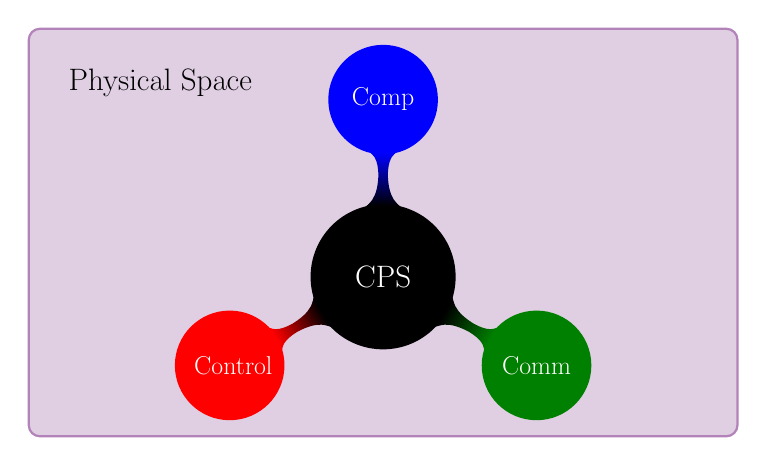
\begin{tikzpicture}[scale=0.45,transform shape,level distance=0cm,
        level 1 concept/.append style={sibling angle=120,minimum size = 3cm},
        ]
        \path [draw=thupurple!50,fill=thupurple!20,thick,rounded corners] (-10,-4.5) rectangle (10,7);
        \node at (-9,6) [anchor=north west] {\Huge Physical Space};
        \path[mindmap,concept color=black,text=white]
        node[concept] {\Huge CPS}
        [clockwise from=330]
        child[concept color=green!50!black] { node[concept](communication) {\huge Comm} }
        child[concept color=red] { node[concept](control) {\huge Control} }
        child[concept color=blue] { node[concept](computation) {\huge Comp} };
      \end{tikzpicture}
    \end{center}
  \item Applications: aerospace, chemical processes, civil infrastructure, energy, manufacturing and transportation. 
  \end{itemize}
\end{frame}

\begin{frame}{Security Threats for the CPS}
  \begin{itemize}
  \item The next generation CPS: Smart Grids, Smart Buildings, Smart Home, Internet of Things, will make extensive use of widespread sensing and networking.
  \item As the CPSs become ``smarter'', they are also more vulnerable to malicious attacks.
  \end{itemize}
  \begin{figure}[ht]
    \centering
    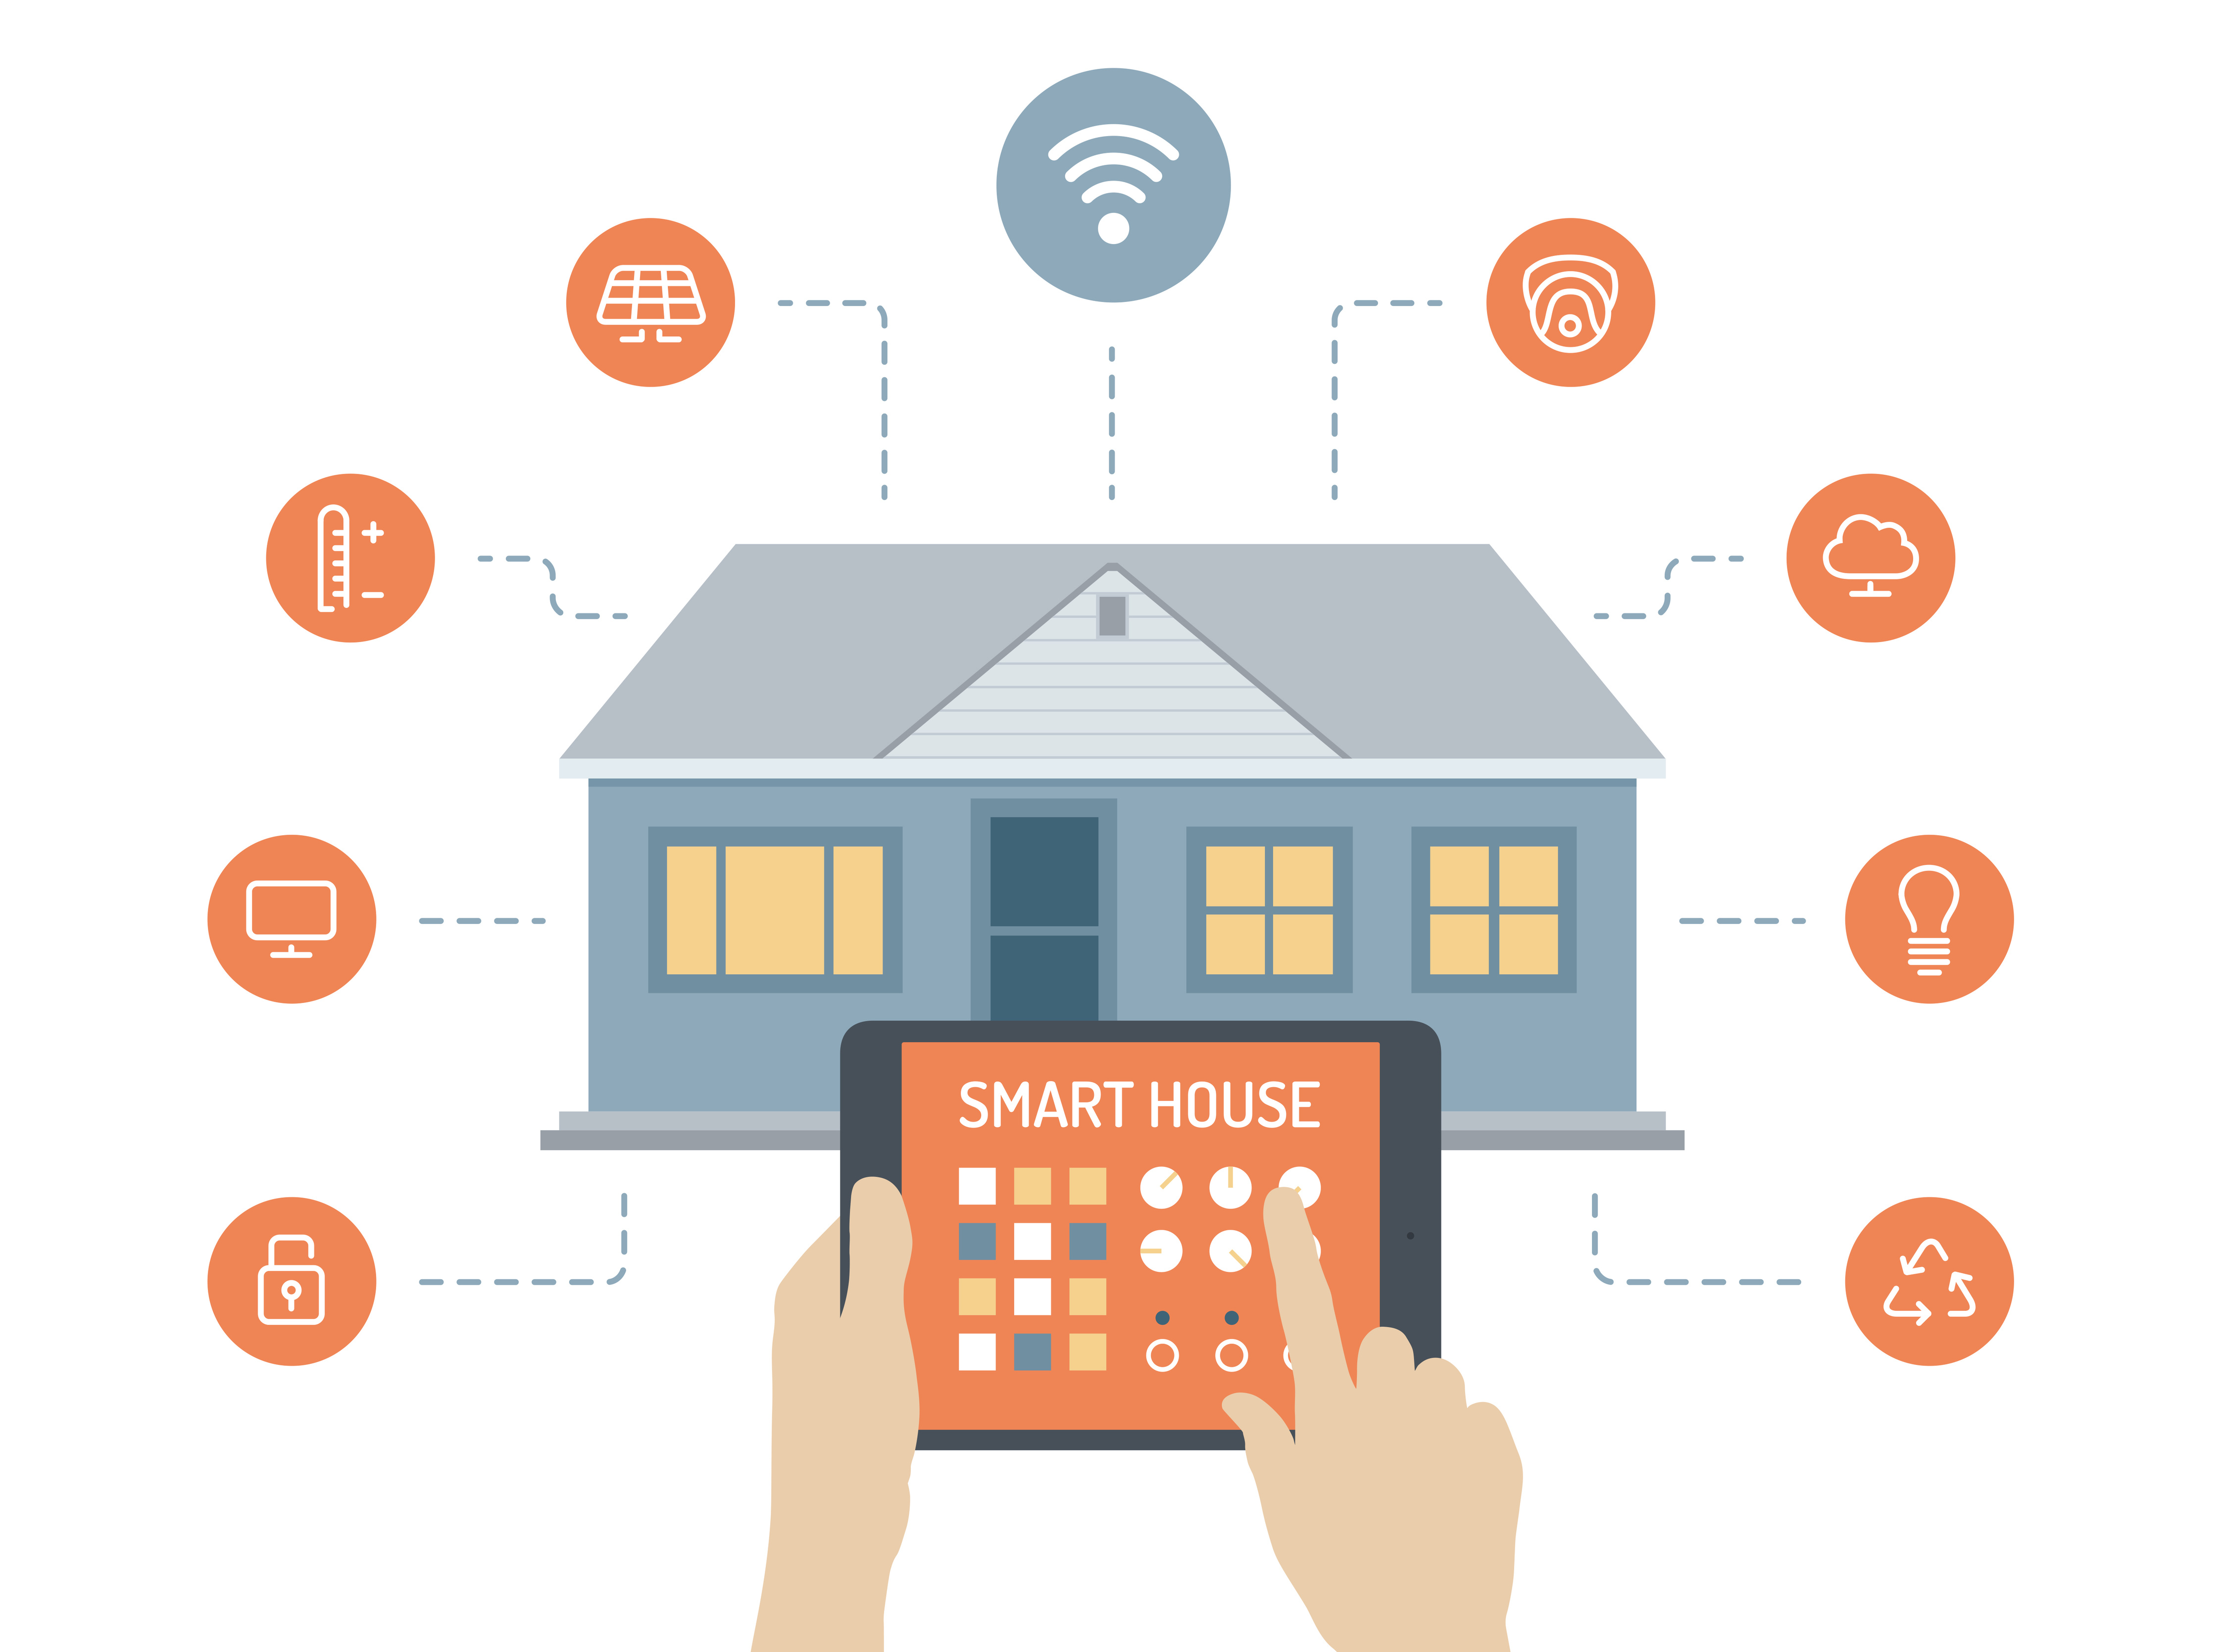
\includegraphics[width=0.6\textwidth]{SmartHome.jpg}
  \end{figure}
\end{frame}

\begin{frame}{Stuxnet}
  \begin{figure}[ht]
    \centering
    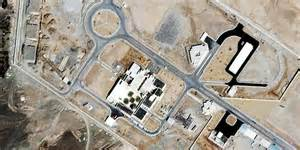
\includegraphics[width=0.8\textwidth]{stuxnet.jpg}
  \end{figure}
  Stuxnet is the first discovered malware that spies on and subverts industrial control systems. It was discovered in June 2010. 
\end{frame}

\begin{frame}{Industrial Control Systems}
  \begin{figure}[ht]
    \centering
    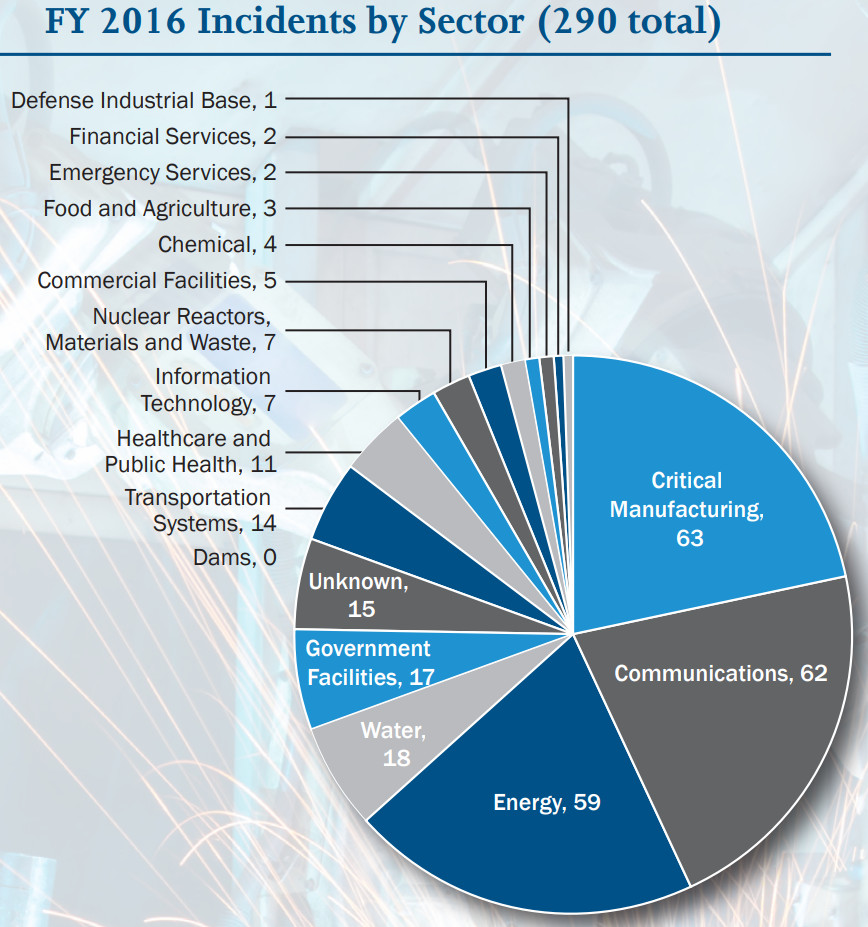
\includegraphics[width=0.6\textwidth]{cert.jpg}
  \end{figure}
 In FY 2014, ICS-CERT (Industrial Control Systems Cyber Emergency Response Team) received and responded to 245 incidents as reported by asset owners and industry partners.
\end{frame}


\begin{frame}{Industrial Control Systems}
   The scope of incidents encompassed a vast range of threats and observed methods for attempting to gain access to both business and control systems infrastructure, including but not limited to the following:
  \begin{enumerate}
  \item  Unauthorized access and exploitation of Internet facing ICS/Supervisory Control and Data Acquisition (SCADA) devices,
  \item 	 Exploitation of zero-day vulnerabilities in control system devices and software, 
  \item  	 Malware infections within air-gapped control system networks,
  \item \dots
  \end{enumerate}

\end{frame}

\begin{frame}{Attack Through Compromised Supply Chain}
  \begin{figure}[ht]
    \centering
    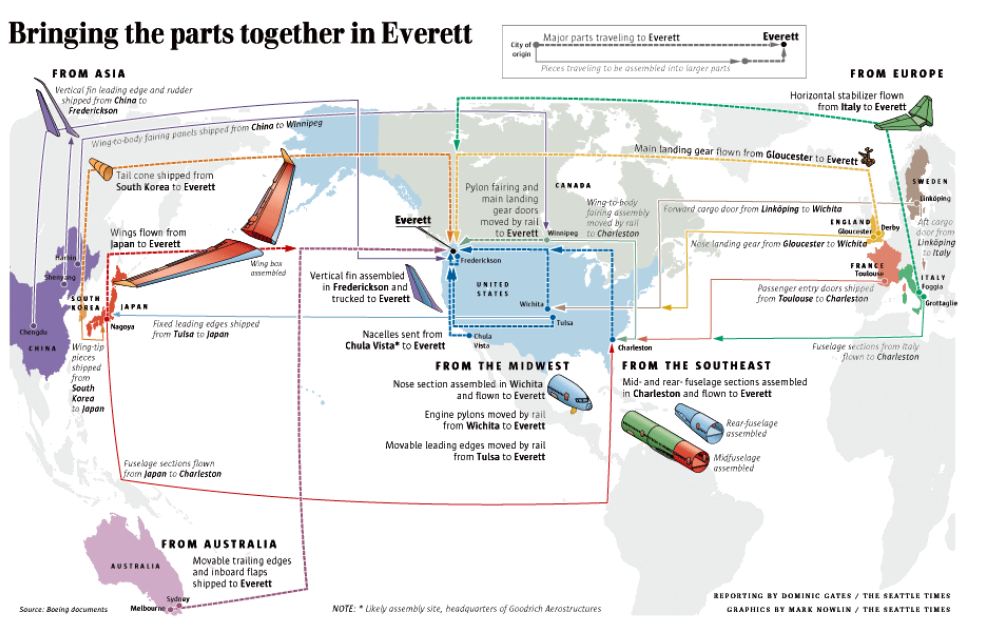
\includegraphics[width=0.8\textwidth]{boeing.jpg}
    \caption{Boeing 787 outsourced 70\% of its parts.}
  \end{figure}
\end{frame}

\begin{frame}{2003 Northeast Blackout}
  \begin{figure}[<+htpb+>]
    \begin{center}
      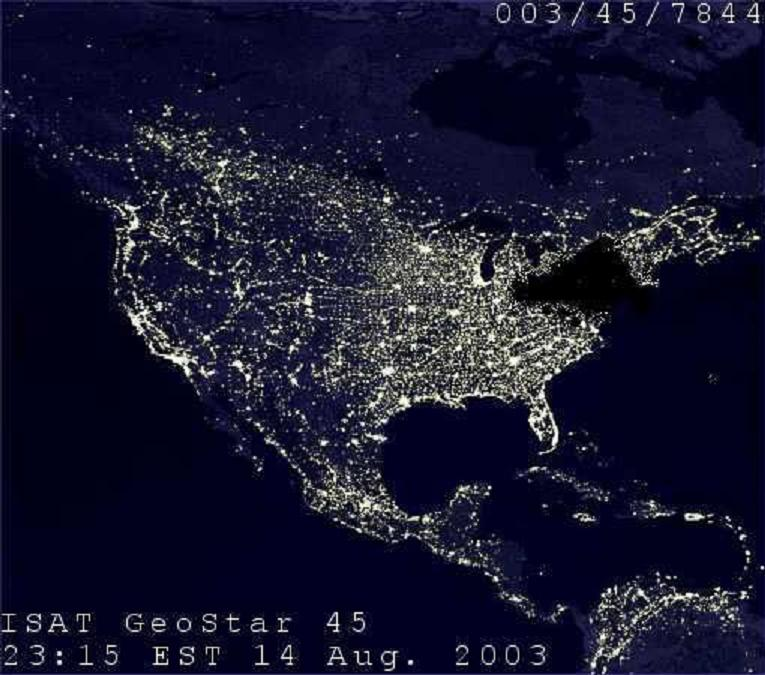
\includegraphics[width=0.60\textwidth]{blackout.jpg}
      \caption{A successful attack on CPS can have devastating effects.}
    \end{center}
  \end{figure}
\end{frame}

%\begin{frame}{How to deal with CPS security threats}
%  \begin{exampleblock}{}
%    {\it `` If you know the enemy and know yourself, you need not fear the result of a hundred battles. If you know yourself but not the enemy, for every victory gained you will also suffer a defeat. If you know neither the enemy nor yourself, you will succumb in every battle.''}
%    \vskip5mm
%    \hspace*\fill{ \small--- The Art of War }
%  \end{exampleblock}
%
%  \begin{enumerate}
%  \item Intrusion detection and isolation
%  \item Information Fusion 
%  \end{enumerate}
%\end{frame}
\section{Physical Watermarking}
\frame{\tableofcontents[currentsection]}

\begin{frame}{Stuxnet}
  \begin{itemize}
    \item NY times:``The worm itself now appears to have included two major components. One was designed to send Iran's nuclear centrifuges spinning wildly out of control. Another seems right out of the movies: The computer program also \alert{secretly recorded what normal operations at the nuclear plant looked like, then played those readings back to plant operators}, like a pre-recorded security tape in a bank heist, so that it would appear that everything was operating normally while the centrifuges were actually tearing themselves apart.''
  \end{itemize}
\end{frame}

\begin{frame}{System Model}
  \begin{block}{System Description}
      \begin{displaymath}
	\begin{split}
	  x(k+1) &= Ax(k)  + Bu(k)+w(k),\\
	  y(k) &= C x(k) + v(k).
	\end{split}
      \end{displaymath}
    \end{block}
    \begin{itemize}
      \item $x(k) \in \mathbb R^n$ is the state vector.
      \item  $y(k) \in \mathbb R^m$ is the measurements from the sensors.
      \item  $u(k) \in \mathbb R^p$ is the control input.
      \item $w(k),v(k),x(0)$ are independent Gaussian random vectors, and $x(0) \sim \mathcal N(0,\;\Sigma)$, $w(k) \sim \mathcal N(0,\;Q)$ and $v(k) \sim \mathcal N(0,\;R)$ with $Q,R>0$.
      \item The system is assumed to be controllable and observable.
    \end{itemize}
  \end{frame}

  \begin{frame}{LQG Controller and Kalman filter}
    \begin{itemize}
      \item We assume that the system operator wants to minimize the following cost function:
	\begin{displaymath}
	  J = \lim_{T\rightarrow \infty}\min_{u(0),\ldots,u(T)}E\frac{1}{T}\left[\sum_{k=0}^{T-1} x(k)'Wx(k)+u(k)'Uu(k)\right],
	\end{displaymath}
	where $W, U$ are positive semidefinite matrices. 
      \item The optimal controller is a fixed gain controller, which takes the following form:
	\begin{displaymath}
	  u(k) =  L^*\hat x(k),
	\end{displaymath}
      \item The optimal estimator (Kalman filter) follows the following update equations:
	\begin{align*}
	  \hat x(k+1|k) &= A\hat x(k)+Bu(k),\\
	  \hat x(k+1) &= \hat x(k+1|k) + K^*\left[y(k+1) - C\hat x(k+1|k)\right],
	\end{align*}
    \end{itemize}
  \end{frame}


  \begin{frame}{$\chi^2$ Failure Detector}
    \begin{itemize}
      \item The residue $z(k)$ of the Kalman filter is defined as
	\begin{displaymath}
	  z(k) \triangleq y(k) - C\hat x(k|k-1),
	\end{displaymath} 
	which is i.i.d. Gaussian distributed with zero mean. 
      \item $\chi^2$ detector triggers an alarm based on the following event:
	\begin{displaymath}
	  g(k)=  z(k)^T\mathcal P^{-1}z(k)> threshold,
	\end{displaymath}
	where $\mathcal P$ is the covariance matrix of $z(j)$ and $\mathcal T$ is the window size.
      \item The alarm rate at time $k$ is 
	\begin{displaymath}
	  \beta(k) = P(g(k) > threshold).
	\end{displaymath}
	If the system is operating normally, then the alarm rate is a constant, which we denote as the false alarm rate $\alpha$.
    \end{itemize}
  \end{frame}

  \begin{frame}{System Diagram}
    \begin{figure}[htpb]
      \begin{center}
	\inputtikz{systemdiagram}
      \end{center}
    \end{figure}
  \end{frame}

  \begin{frame}{Replay Attack Model}
    \begin{enumerate}
      \item The attacker can read and modify all the measurements $y(k)$ arbitrarily.
      \item It can inject an external control input $u^a(k)$ into the system. 
    \end{enumerate}
    The strategy of the attacker can be divided into two stages:
    \begin{enumerate}
      \item The attacker records a sufficient number of $y(k)$s without injecting any control input $u^a(k)$. 
      \item The attacker injects a sequence of desired control input $u^a(k)$ while replaying the previous recorded $y(k)$s starting from time $0$.
    \end{enumerate}
    When the system is under attack, the controller will be unable to perform closed-loop control. Hence the only way to counter this attack is to detect its presence. 
  \end{frame}

  \begin{frame}{Replay Attack: First Stage}
    \begin{figure}[htpb]
      \begin{center}
	\inputtikz{replaydiagramone}
      \end{center}
    \end{figure}
  \end{frame}

  \begin{frame}{Replay Attack: Second Stage}
    \begin{figure}[htpb]
      \begin{center}
	\inputtikz{replaydiagramtwo}
      \end{center}
    \end{figure}
  \end{frame}

  \begin{frame}{Feasibility of Replay Attacks}
    \begin{figure}[htpb]
      \setlength\figureheight{4.5cm}
      \setlength\figurewidth{10cm}
      \begin{center}
	\inputtikz{replayunstableA2}
      \end{center}
    \end{figure}
    Replay attack is not always feasible!
  \end{frame}

  \begin{frame}{Feasibility of Replay Attacks}
    \begin{figure}[htpb]
      \begin{center}
	\inputtikz{replaydiagramthree}
      \end{center}
    \end{figure}
  \end{frame}

  \begin{frame}{Feasibility of Replay Attacks}
    The update equation of Kalman filter follows:
    \begin{align*}
      \hat{x}(k+1|k)&=A\hat{x}(k)+Bu(k)=\left(A+BL^*\right)\hat{x}(k)\\
      &=\left(A+BL^*\right)\left(I-K^*C\right)\hat{x}(k|k-1)+\left(A+BL^*\right)K^*y(k).
    \end{align*}

    \begin{theorem}
      If $\mathcal A = (A+BL^*)(I-K^*C)$ is stable, then the detection rate of $\chi^2$ detector $\beta^c(k)$ converges to the false alarm rate $\alpha$ during the attack, i.e.,
      \begin{displaymath}
	\lim_{k\rightarrow\infty}\beta^c(k) = \alpha.  
      \end{displaymath}
      On the other hand, if $\mathcal A$ is strictly unstable, then the detection rate $\beta^c(k)$ converges to $1$, i.e.,
      \begin{displaymath}
	\lim_{k\rightarrow\infty}\beta^c(k) = 1.  
      \end{displaymath}
    \end{theorem}
  \end{frame}

  \begin{frame}{Countermeasures: Authentication and Watermarking}
    \begin{itemize}
      \item Challenge-response authentication is widely in cyber security, where one party presents a question ("challenge") and another party must provide a valid answer ("response") to be authenticated.
      \item Similarly, we could change the control law by adding a random watermarking signal:
	\begin{displaymath}
	  u(k) = L^*\hat x(k) + \zeta(k).
	\end{displaymath}
      \item The watermarking signal $\zeta(k)$ acts as a ``challenge'' and the sensor measurement is the ``response''. 
      \item During normal operation, the ``challenge'' and ``response'' are correlated through the system dynamics, while the correlation cease to exist when the replay begins.
      \item The CPS will remain stable. However, we sacrifice LQG performance since the control is not optimal.
      \item How to design the ``optimal'' watermarking signal?
    \end{itemize}
  \end{frame}

  \begin{frame}{Countermeasures: Authentication and Watermarking}
    \begin{itemize}
      \item We restrict the watermarking signal $\zeta(k)$ to be a zero-mean i.i.d. Gaussian process generated with covariance $U$.
      \item The additional LQG cost incurred by $\zeta(k)$ is a linear function of $U$.
	\begin{displaymath}
	  \text{Additional LQG cost} = \tr(U\mathcal X).
	\end{displaymath}
      \item The KL divergence between ``compromised'' residue $z^c(k)$ and ``normal'' residue $z(k)$ is a convex functional $U$, which satisfies
	\begin{displaymath}
	  \frac{1}{2}\tr(U\mathcal P) \leq D_{KL}(z^c(k)||z(k))\leq \tr(U\mathcal P)-\frac{1}{2}\log(1+\tr(U\mathcal P)).
	\end{displaymath}
        Both the upper and lower bounds are increasing functions of $\tr(U\mathcal P)$.
    \end{itemize}
  \end{frame}

  \begin{frame}{Countermeasures: Authentication and Watermarking}
    We consider maximizing the ``relaxed'' KL divergence, while satisfying LQG performance constraint.
    \begin{align*}
      &\mathop{\textrm{maximize}}\limits_{U}&
      & \tr (U\mathcal P)\\
      &\textrm{subject to}&
      & \tr (U\mathcal X) \leq \delta \\
      &&& U \text{ is positive semidefinite.}
    \end{align*}
    Given matrices $\mathcal P$ and $\mathcal X$, one can prove that $U = \alpha v v^T$ is a rank $1$ matrix, where $v$ is a generalized eigenvector of $\mathcal P,\mathcal X$ and $\alpha >0$ is chosen such that $ \alpha v^T\mathcal X v =\delta$.
  \end{frame}

  \begin{frame}{Learning Based Watermarking Design}
    \begin{itemize}
    \item If we know all system parameters precisely, the watermarking signal design and detector design is trivial.
    \item What if we do not know the parameters or only know rough estimates of the parameters?
    \item We design a mechanism to combine system identification and watermarking design, assuming that we only knows the dimension of the system $n$.
    \end{itemize}
  \end{frame}

  \begin{frame}{Tennessee Eastman Process}
    Here, we apply the proposed technique to the Tennessee Eastman Process (TEP).\\~\\
    \begin{itemize}
    \item The TEP is created to provide a realistic industrial process for developing studying and evaluating process control technology. 
    \item The Tennessee Eastman (TE) problem requires coordination of three unit operations: an exothermic, two-phase reactor, a flash separator and a reboiled  stripper.
    \item There are 41 measured output variables (with added measurement noise) and 12 manipulated variables.
    \item The original TE problem is very complex and the accurate model equations are not given by Eastman Chemical Company.   
    \end{itemize}
  \end{frame}

  \begin{frame}{Simplified TEP Model}
    Ricker (1993) proposed the following simplified TEP. The total volume is fixed. The reaction in the vapor phase is: $A+C\rightarrow D$.
    \begin{columns}
      \begin{column}{0.45\textwidth}
        \begin{figure}
          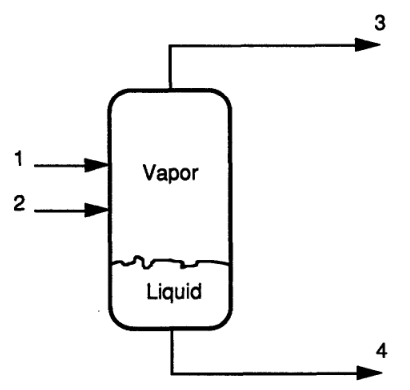
\includegraphics[width=0.9\textwidth]{simplifiedmodel.png}
          \caption{The simplified process}
        \end{figure}
      \end{column}
      \begin{column}{0.55\textwidth} 		
        \begin{itemize}
        \item The vessel: a combination of the reactor and separation system in the original TE Process;
        \item Feed 1: A, C and trace amounts of an inert B;
        \item Feed 2: pure A;
        \item Stream 3: purge rate;
        \item Stream 4: product rate;
        \item Vapor: A, B, C;\\
          Liquid: D.
        \end{itemize}
      \end{column}
    \end{columns}
  \end{frame}

  \begin{frame}{Simplified TEP Model}
    Ricker (1993) also provided a LTI dynamic model of the plant, and a corresponding robust controller with 4 outputs and 4 inputs.
    \begin{block}{Simplified transfer-function model}
      \begin{align*}
        \textbf{y}= \begin{bmatrix}
          F_4\\ 
          P\\ 
          y_{A3}\\
          V_L 
        \end{bmatrix}=\textbf{G}\textbf{u}=\begin{bmatrix}
          g_{11} & 0 & 0 & g_{14}\\ 
          g_{21} & 0 & g_{23} & 0\\ 
          0 & g_{32} & 0 & 0\\ 
          0 & 0 & 0 & g_{44} 
        \end{bmatrix}\begin{bmatrix}
          u_1\\ 
          u_2\\ 
          u_3\\ 
          u_4
        \end{bmatrix}
      \end{align*}
      For this model:\\
      \begin{itemize}
      \item Four manipulated variables: changes of the $i$th valve position.
      \item Four output variables: $F_4$: production rate, $P$: pressure,\\ $y_{A3}$: amount of A in purge, $V_L$: liquid inventory. 
      \item The individual transfer functions: $g_{11},\, g_{14},\, g_{21},\, g_{32},\, g_{44}$ and $g_{23}$ are also given. 
      \end{itemize}
    \end{block}
  \end{frame}

  \begin{frame}{Simulation Results}
    We apply the proposed technique to the simplified version of TE Process. \\~\\

    Discretizing the simplified TEP model with sampling period $T_{sp} = 0.6s$, we can derive the system matrices $A$, $B$ and $C$, where  
    \begin{itemize}
    \item $A$, $B$ and $C$ are sparse matrices.
    \item The eigenvalues of A is 0.9418,  0.9418, 0.5488, 0.5488, 0.4493, 0.0907, 0.0025. 
    \end{itemize}
    ~\\
    This system simulates a MIMO system with order $n = 7$ with  $p = 4$ inputs and $m = 4$ outputs. Moreover, the covariance matrices $Q = I_{7}$ and $ R = I_{4}$, $X = I_{8}$,  $\delta = 15$ ($13.13\%$ of the LQG cost $J = 114.22$), $\beta = \frac{1}{3}$.
  \end{frame}

  \begin{frame}
    \frametitle{The Watermark Signal Design}
    \begin{columns}
      \begin{column}{0.6\textwidth}
        \begin{figure}[h!]
          \inputtikz{errU1_te}
        \end{figure}
      \end{column}
      \begin{column}{0.4\textwidth}
        \begin{itemize}
        \item  $k^*$ denotes the update times, the update interval is $100$;
        \item $U$: the optimal covariance of the watermark signal;
        \item $U_k$: the estimation of $U$.
        \end{itemize}
      \end{column}
    \end{columns}
    ~\\
    As time $k^*$ goes to infinity, $U_k$ converges to the optimal covariance of the watermark signal, $U$.
  \end{frame}

  \begin{frame}
    \frametitle{The detection performance}
    \begin{itemize}
    \item $g_n$: the output of the $\chi^2$ detector designed with know parameters
    \item $g$: the output of the $\chi^2$ detector when the parameters of the system are inferred through the learning technique. 
    \end{itemize}
    \begin{figure}[h!]
      \centering
      \inputtikz{gng_te}
    \end{figure}
  \end{frame}

  \section{Privacy Preserving Consensus}
  \begin{frame}{Centralized v.s. Distributed Algorithm}
    \begin{figure}[<+htpb+>]
      \begin{center}
        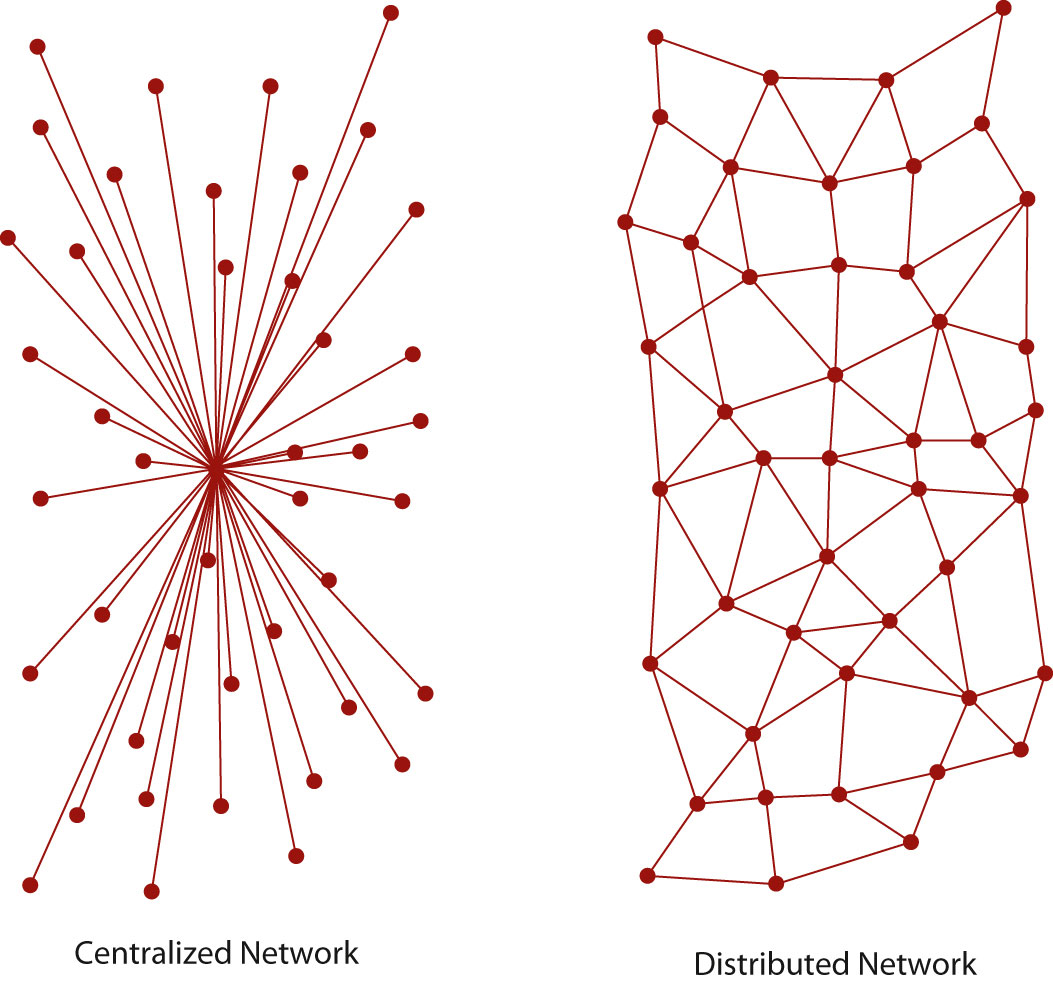
\includegraphics[width=0.50\textwidth]{centralized.jpg}
      \end{center}
    \end{figure}
    Benefit of distributed algorithm: Reliability, Scalability, Transparency, Incremental Growth, Privacy
  \end{frame}

  \begin{frame}{Preliminary: Average Consensus}
    \begin{itemize}
    \item We model the network composed of $n$ agents as an \emph{undirected} and \emph{connected} graph $G = \{V,\,E\}$.
    \item Define the neighborhood of sensor $i$ as $\mathcal N(i)$.
    \item Each agent has an initial scalar state $x_{i}(0)$.
    \item Update equation:
      \begin{displaymath}
        x_i(k+1) = a_{ii} x_{i}(k) + \sum_{j\in \mathcal N(i)} a_{ij} x_{j}(k).  
      \end{displaymath}
    \item Update equation in matrix form:
      \begin{displaymath}
        x(k+1) = A x(k),
      \end{displaymath}
      where we assume that $A$ is \emph{symmetric}.
    \end{itemize}
  \end{frame}

  \begin{frame}{Preliminary: Average Consensus}
    Define the average vector as
    \begin{displaymath}
      \bar x\triangleq \frac{\mathbf 1' x(0)}{n} \mathbf 1.
    \end{displaymath}
    The following conditions are necessary and sufficient for all the agents to reach average consensus:
    \begin{enumerate}
    \item[(A1)] $ \lambda_1 = 1$ and  $|\lambda_i| < 1$ for all $i = 2,\ldots, n$.
    \item[(A2)] $A\mathbf 1 = \mathbf 1$, i.e., $\mathbf 1$ is an eigenvector of $A$.
    \end{enumerate}
  \end{frame}

  \begin{frame}{Applications of Consensus}
    \begin{itemize}
    \item Dynamic load balancing;
    \item Vehicle formation control;
    \item Rendezvous problem;
    \item Social network;
    \item Clock Synchronization;
    \item Localization;
    \item Distributed Estimation;
    \item Distributed Optimization;
    \item \dots
    \end{itemize}
  \end{frame}

  \begin{frame}{Challenges}
    \begin{itemize}
    \item Malicious Attacker: What if some agent do not follow the update rule:
      \begin{displaymath}
        x_i(k+1) = a_{ii} x_{i}(k) + \sum_{j\in \mathcal N(i)} a_{ij} x_{j}(k).  
      \end{displaymath}

      \emph{(Pasqualetti, Bicchi and Bullo, 2012)}: If there are $k$ malicious agents, then
      \begin{itemize}
      \item a benign node can detect the presence of malicious agents if the size of the minimum cut of the graph is at least $k + 1$.
      \item a benign node can identify the set of the malicious agents if the size of the minimum cut of the graph is at least $2k + 1$.
      \end{itemize} 

    \item Curious Attacker: What if an agent wants to infer the initial state of other agents?
    \item Malicious \& Curious Attacker?: Separation principle.
    \end{itemize}
  \end{frame}

  \begin{frame}{Privacy Concerns}
    \begin{itemize}
    \item Without loss of generality, we consider agent $n$ wants to estimate the initial states of other agents.
    \item Denote the neighborhood of agent $n$ as
      \begin{displaymath}
        \mathcal N(n) = \{j_1,\dots,j_m\}.
      \end{displaymath}
    \item Define
      \begin{displaymath}
        \begin{split}
          C &\triangleq \begin{bmatrix}
            e_{j_1}&\dots&e_{j_m}&e_n
          \end{bmatrix}' \in \mathbb R^{(m+1)\times n},\\
          y(k)&\triangleq \begin{bmatrix}x_{j_1}(k)&\dots&x_{j_m}(k)&x_n(k)
          \end{bmatrix}=Cx(k).
        \end{split}
      \end{displaymath}
    \item The information set for agent $n$ at time $k$ is 
      \begin{displaymath}
        \mathcal I(k) = \{y(0),\dots,y(k)\}. 
      \end{displaymath}
    \end{itemize}
  \end{frame}

  \begin{frame}{Privacy Concerns}
    For agent $n$, the problem becomes a standard estimation problem of the following linear system: 
    \begin{displaymath}
      x(k+1) = A x(k),\,y(k) = C x(k). 
    \end{displaymath}
    Since the system is noiseless, if $x_i$ is in the observable space of $(A,C)$, then agent $n$ can perfectly recover the initial state $x_i(0)$ of agent $i$. 

    \alert{The privacy of agent $i$ is breached.}
  \end{frame}

  \begin{frame}{Example}
    \begin{center}
      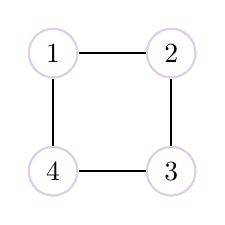
\begin{tikzpicture}
        \node (n4) at (0,0) [circle,draw=thupurple!50,draw=thupurple!20,thick] {4};
        \node (n1) at (0,1.5cm) [circle,draw=thupurple!50,draw=thupurple!20,thick] {1};
        \node (n3) at (1.5cm,0) [circle,draw=thupurple!50,draw=thupurple!20,thick] {3};
        \node (n2) at (1.5cm,1.5cm) [circle,draw=thupurple!50,draw=thupurple!20,thick] {2};
        \draw [semithick] (n1)--(n2)--(n3)--(n4)--(n1);
      \end{tikzpicture}
    \end{center}
    \begin{enumerate}
    \item At time step $0$, agent $4$ knows $x_1(0)$ and $x_3(0)$.
    \item At time step $1$, agent $4$ knows $x_1(1)$, which is
      \begin{align*}
        x_1(1) = a_{11}x_1(0)+a_{14}x_4(0)+a_{12}x_2(0).    
      \end{align*}
    \end{enumerate}

    For agent $4$, it can infer all the initial state $x(0)$ in two steps.

  \end{frame}


  \begin{frame}{Privacy Preserving Average Consensus}
    \begin{enumerate}
    \item At time $k$, each agent generates a standard normal distributed random variable $v_i(k)$ with mean $0$ and variance 1. We assume that all the random variables $\{v_i(k)\}_{i=1,\dots,n,\,k=0,1,\dots}$ are jointly independent.
    \item Each agent then adds a random noise $w_i(k)$ to its state $x_i(k)$, where
      \begin{displaymath}
        w_i(k) = \begin{cases}
          v_i(0)&\text{, if }k = 0\\
          \varphi^kv_i(k)-\varphi^{k-1}v_i(k-1)&\text{, otherwise}
        \end{cases},
        \label{eq:addednoise}
      \end{displaymath}
      where $0<|\varphi|<1$ is a constant for all agents. Define the new state to be $x_{i}^+(k)$, i.e.,
      \begin{displaymath}
        x_{i}^+(k) = x_i(k) + w_i(k).  
        \label{eq:noisestep}
      \end{displaymath}
    \item Each agent then communicates with its neighbors and update its state to the average value, i.e.,
      \begin{displaymath}
        x_i(k+1) = a_{ii}x_i^+(k)+\sum_{j\in \mathcal N(i)}a_{ij}x_{j}^+(k).
        \label{eq:consensusstep}
      \end{displaymath}
    \item There is no requirement for additional communication.
    \end{enumerate}
  \end{frame}

  \begin{frame}{Privacy Preserving Average Consensus}
    \begin{figure}[ht]
      \begin{center}
        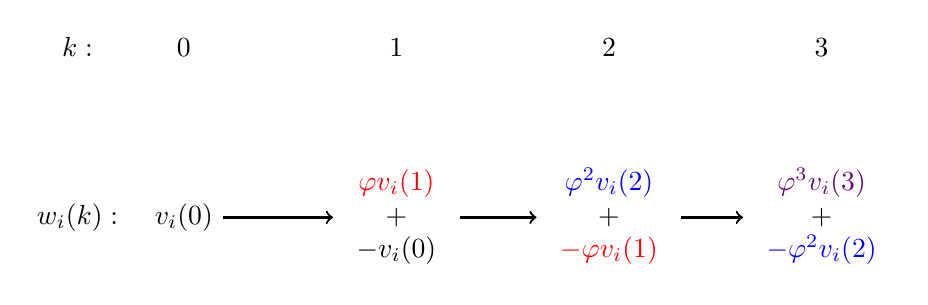
\begin{tikzpicture}[scale=0.9]
          \node [label=above:$k:$] at (-1.5,0) {};
          \node [label=above:$0$] at (0,0) {};
          \node [label=above:$1$] at (3,0) {};
          \node [label=above:$2$] at (6,0) {};
          \node [label=above:$3$] at (9,0) {};
          \node [] at (-1.5,-2) {$w_i(k):$};
          \node [] (n0) at (0,-2){$v_i(0)$}; 
          \node [] (n1) at (3,-2){$\begin{array}{c}\textcolor{red}{\varphi v_i(1)}\\+\\- v_i(0)\end{array}$}; 
          \node [] (n2) at (6,-2){$\begin{array}{c}\textcolor{blue}{\varphi^2 v_i(2)}\\+\\\textcolor{red}{- \varphi v_i(1)}\end{array}$}; 
          \node [] (n3) at (9,-2){$\begin{array}{c}\textcolor{thupurple}{\varphi^3 v_i(3)}\\+\\\textcolor{blue}{ -\varphi^2 v_i(2)}\end{array}$}; 
          \draw [->,thick] (n0)--(n1);
          \draw [->,thick] (n1)--(n2);
          \draw [->,thick] (n2)--(n3);
        \end{tikzpicture}
      \end{center}
    \end{figure}
  \end{frame}

  \begin{frame}{Privacy Preserving Average Consensus}
    \begin{itemize}
    \item Update equation in matrix form:
      \begin{displaymath}
        x(k+1) =Ax^+(k)= A(x(k) + w(k)).
      \end{displaymath}
    \item Agent $n$ only receives a noisy version of the state:
      \begin{displaymath}
        y(k) = C x^+(k) = C(x(k)+w(k)).	
      \end{displaymath}
    \end{itemize}
  \end{frame}

  \begin{frame}{Performance Metric}
    Define the error vector as
    \begin{displaymath}
      e(k) \triangleq x(k) - \bar x.
    \end{displaymath}
    Define the mean square convergence rate as
    \begin{displaymath}
      \rho \triangleq \limsup_{k\rightarrow\infty} \left( \sup_{z(0)\neq 0}\frac{\mathbb E_v e(k)'e(k)}{e(0)'e(0)}\right)^{1/k},
    \end{displaymath}
  \end{frame}

  \begin{frame}{Performance Metric}
    \begin{itemize}
    \item The new information set of agent $n$ at time $k$ is
      \begin{displaymath}
        \mathcal I(k) \triangleq \{x_n(0),y(0),\dots,y(k)\}.
      \end{displaymath}
    \item Denote the maximum likelihood estimate of $x(0)$ given $\mathcal I(k)$ as $\hat x(0|k)$, the covariance of which is defined as $P(k)$.

    \item  Clearly, $\mathcal I(k)\subset \mathcal I(k+1)$, which implies $P(k)\geq P(k+1)$. Hence, we can define

      \begin{displaymath}
        P = \lim_{k\rightarrow\infty} P(k). 
      \end{displaymath}

      $P$ is best estimation performance that can be achieved by agent $n$ (with infinite observations).

    \item If $P_{ii} = 0$, then agent $n$ can infer the initial state $x_i(0)$ of agent $i$ without any error (asymptotically).

    \end{itemize}
    Our goal is to make $\rho$ \emph{small}, while making $P$ \emph{large}.
  \end{frame}

  \begin{frame}{Convergence Result}
    \begin{theorem}
      For any initial condition $x(0)$, $x(k)$ converges to $\bar x$ in the mean square sense. Furthermore, the mean square convergence rate $\rho$ equals
      \begin{displaymath}
        \rho = \max(|\varphi|^2,|\lambda_2|^2,|\lambda_n|^2).
      \end{displaymath}
    \end{theorem}
    If we choose $\varphi$ to be small enough, then the added noise will not deteriorate the consensus speed.
  \end{frame}

  % \begin{frame}{Reduced System}
  %   \begin{itemize}
  %   \item Define $\tilde x(k) = \begin{bmatrix} x_1(k)&\dots&x_{n-1}(k) 
  %     \end{bmatrix}$. 
  %   \item $\tx(k)$ follows:
  %     \begin{displaymath}
  %       \tx(k+1) = \tA \tx^+(k) + \zeta x_n^+(k),
  %     \end{displaymath}
  %     where $\tA\in \mathbb R^{(n-1)\times(n-1)}$ is the principal minor of $A$ by removing the last row and column
  %   \item Similarly, we can define
  %     \begin{displaymath}
  %       \ty = \begin{bmatrix}\tx^+_{j_1}(k)&\dots&\tx^+_{j_m}(k)
  %       \end{bmatrix} = \tC \tx^+(k) .
  %     \end{displaymath}
  %   \item We assume that $(\tA,\tC)$ is observable, otherwise we can do a Kalman decomposition and only consider the observable space.
  %   \end{itemize}
  % \end{frame}
  % 
  % \begin{frame}{Reduced System}
  %   \begin{theorem}
  %     $\tilde A$ is strictly stable, i.e., $\|\tA\|<1$. 
  %   \end{theorem}
  %   \begin{itemize}
  %   \item Consider the following $n-1$ by $n-1$ symmetric matrix
  %     \begin{displaymath}
  %       \mathcal S = (I-\tA)^{-1}\tC'\tC(I-\tA)^{-1}
  %     \end{displaymath}
  %   \item $I-\tA$ is invertible, $\tC$ is of rank $m$. Hence $\rank(\mathcal S) = m$. 
  %   \item Let $\psi_1,\dots,\psi_{n-1}\in \mathbb R^{n-1}$ be the eigenvectors of $\mathcal S$. 
  %   \item Assume that the eigenvalues corresponding to $\{\psi_1,\dots,\psi_m\}$ are non-zero and the eigenvalues corresponding to $\{\psi_{m+1},\dots,\psi_{n-1}\}$ are zero. 
  %   \item Define
  %     \begin{align}
  %       \mathcal Q_1&\triangleq \begin{bmatrix}
  %         \psi_1&\dots&\psi_m
  %       \end{bmatrix}\in \mathbb R^{(n-1)\times m},\\
  %       \mathcal Q_2& \triangleq \begin{bmatrix}
  %         \psi_{m+1}&\dots&\psi_{n-1}
  %       \end{bmatrix}\in \mathbb R^{(n-1)\times (n-m-1)}.
  %     \end{align}
  %   \end{itemize}
  % \end{frame}

  \begin{frame}{Estimation Performance}
    \begin{theorem}
      Suppose that $0<\varphi<1$. $P$ is given by the following equality:
      \begin{displaymath}
        P =\begin{bmatrix}
          \mathcal Q_2\left[\mathcal Q_2'(I-\tA)^{-1}Y(I-\tA)^{-1}\mathcal Q_2\right]^{-1} \mathcal Q_2'&\mathbf 0\\
          \mathbf 0'&0
        \end{bmatrix}
      \end{displaymath}
      where $ Y = \lim_{k\rightarrow\infty} Y(k)$ is the limit of the following recursive Riccati equations:
      \begin{align*}
        Y(0)& = \tA \mathcal U \tA,\\
        Y(k+1) &=\tA \mathcal U\tA  +\varphi^{-2}\tA&\left[ Y^+(k) -  Y^+(k)\left(\varphi^2 I+Y^+(k) \right)^{-1}Y^+(k)\right]\tA,
      \end{align*}
      where
      \begin{displaymath}
        Y^+(k) = \mathcal V Y(k) \mathcal V.
      \end{displaymath}
    \end{theorem}
  \end{frame}

  % \begin{frame}{Estimation Performance}
  %   \begin{theorem}[Cont.]
  %     Furthermore, the following inequalities hold:
  %     \begin{displaymath}
  %       \left( 1+\frac{\|\tA\|}{\varphi}\right)^{-2} \begin{bmatrix}
  %         \Delta &\mathbf 0\\
  %         \mathbf 0'&0
  %       \end{bmatrix}\leq P \leq \left( 1-\frac{\|\tA\|}{\varphi}\right)^{-2} \begin{bmatrix}
  %         \Delta &\mathbf 0\\
  %         \mathbf 0'&0
  %       \end{bmatrix}
  %     \end{displaymath}
  %     where
  %     \begin{displaymath}
  %       \Delta \triangleq \mathcal Q_2\left[\mathcal Q_2'(I-\tA)^{-1}\mathcal X(I-\tA)^{-1}\mathcal Q_2\right]^{-1} \mathcal Q_2',
  %     \end{displaymath}
  %     and $\mathcal X$ is the unique solution of the following Lyapunov equation
  %     \begin{displaymath}
  %       \mathcal X = \tA \mathcal X\tA /\varphi^2+  \tA\tC'\tC\tA . 
  %     \end{displaymath}
  %   \end{theorem}
  % \end{frame}
  \begin{frame}{Estimation Performance}
    Define the essential neighborhood of sensor $i$ as 
    \begin{displaymath}
      \mathcal N_e(i) \triangleq \{j\in V:j\neq i,\,a_{ij}\neq 0\}.
    \end{displaymath}
    Node $j$ is called a super neighbor of $i$ if
    \begin{enumerate}
    \item $j$ is a neighbor of $i$.
    \item $j$ is also a neighbor of all $i$'s essential neighbors.
    \end{enumerate}

    \begin{theorem}
      The $i$th node's privacy is breached to node $j$ if and only if $j$ is a super neighbor of $i$.
    \end{theorem}
    The condition is can be checked \alert{locally}. In other words, your initial state can only be leaked to your neighbors.
  \end{frame}
  \begin{frame}{Estimation Performance}
    \begin{center}
      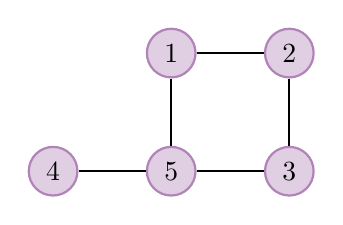
\begin{tikzpicture}
        \node (n4) at (-1.5cm,0) [circle,draw=thupurple!50,fill=thupurple!20,thick] {4};
        \node (n5) at (0,0) [circle,draw=thupurple!50,fill=thupurple!20,thick] {5};
        \node (n1) at (0,1.5cm) [circle,draw=thupurple!50,fill=thupurple!20,thick] {1};
        \node (n3) at (1.5cm,0) [circle,draw=thupurple!50,fill=thupurple!20,thick] {3};
        \node (n2) at (1.5cm,1.5cm) [circle,draw=thupurple!50,fill=thupurple!20,thick] {2};
        \draw [semithick] (n5)--(n1)--(n2)--(n3)--(n5)--(n4);
      \end{tikzpicture}
    \end{center}
    \begin{displaymath}
      \mathcal N(5)\bigcup \{5\} = \{1,3,4,5\}. 
    \end{displaymath}
    \begin{displaymath}
      \mathcal N(4)\bigcup \{4\} = \{4,5\}. \text{ Agent 5 can perfectly infer }x_4(0).
    \end{displaymath}
    \begin{displaymath}
      \mathcal N(1)\bigcup \{1\} = \{1,2,5\}.\text{ Agent 5 cannot perfectly infer }x_1(0)\text{ if }a_{12}\neq 0. 
    \end{displaymath}
  \end{frame}

  % \begin{frame}{Estimation Performance}
  %   \begin{center}
  %     \begin{tikzpicture}
  %       \node (n4) at (0,0) [circle,draw=caltechcolor!50,fill=caltechcolor!20,thick] {4};
  %       \node (n1) at (0,1.5cm) [circle,draw=caltechcolor!50,fill=caltechcolor!20,thick] {1};
  %       \node (n3) at (1.5cm,0) [circle,draw=caltechcolor!50,fill=caltechcolor!20,thick] {3};
  %       \node (n2) at (1.5cm,1.5cm) [circle,draw=caltechcolor!50,fill=caltechcolor!20,thick] {2};
  %       \draw [semithick] (n1)--(n2)--(n3)--(n4)--(n1);
  %     \end{tikzpicture}
  %   \end{center}
  %   Assume $a_{ii} = a_{ij} = 1/3$, then agent $4$ can perfectly recover
  %   \begin{displaymath}
  %     x_4(0),\,x_1(0) + x_2(0) + x_3(0),\,x_1(0) - x_3(0).
  %   \end{displaymath}
  %   However, agent $4$ cannot infer $x_1(0)$, $x_2(0)$, $x_3(0)$ perfectly.
  % \end{frame}

  \begin{frame}{Fundamental Limitation}
    \begin{itemize}
    \item If $P_{ii}=0$ using our average consensus algorithm, it is possible to design another noise sequence $\{w_i(k)\}$ to make $P_{ii}\neq 0$?

    \item Consider a more general noise model:
      \begin{enumerate}
      \item $\mathbb Ew_i(k) = 0$.
      \item $\mathbb Ew_i(k_1)w_j(k_2) = 0$, when $i\neq j$.
      \end{enumerate}
    \item The second condition implies that the sensors are not collaborating.
    \end{itemize}
  \end{frame}

  \begin{frame}{Fundamental Limitation}
    \begin{theorem}
      $x(k)$ converges to $\bar x$ in the mean squared sense, i.e.,
      \begin{displaymath}
        \lim_{k\rightarrow\infty}\mathbb E  \,\|x(k)-\bar x\|^2 = 0,
      \end{displaymath}
      implies that for each agent $i$:
      \begin{displaymath}
        \lim_{k\rightarrow\infty}\mathbb E \,\left(\sum_{t=0}^k w_i(t)\right)^2  = 0, \,\forall i=1,\dots,n.
      \end{displaymath}

    \end{theorem}
    Since the sensors are not collaborating, average consensus is achieved if and only if the noise from each sensor sums to 0 asymptotically (in the mean squared sense).
  \end{frame}

  \begin{frame}{Fundamental Limitation}
    \begin{theorem}
      Suppose that
      \begin{align*}
        \lim_{k\rightarrow\infty}\mathbb E \,\left(\sum_{t=0}^k w_i(t)\right)^2  = 0, \,\forall i=1,\dots,n.
      \end{align*}
      Then $i$th node's privacy is breached to node $j$ \emph{if} $j$ is a super neighbor of $i$.
    \end{theorem}

    Comparing it to the previous theorem, we know that our proposed strategy achieves ``minimum'' privacy breach.
  \end{frame}

  %% \subsection{Differential Privacy}
  %% \begin{frame}{Differential Privacy}
  %%   \begin{itemize}
  %%   \item Denote the probability space generated by $\{v_i(k)\}$ as $(\Omega,\mathcal F,\mathbb P)$.
  %%   \item Define $D = \mathbb R^n$ as the set of all possible initial condition $x(0)$.
  %%   \item  Define a binary ``adjacency'' relation $\text{Adj}$ on $D$:
  %%     \begin{displaymath}
  %%       \text{Adj}(x^a(0),x^b(0)) \triangleq \begin{cases}
  %%         1& \text{, if }\|x^a(0)-x^b(0)\|\leq d\\
  %%         0&\text{, otherwise}
  %%       \end{cases}.
  %%     \end{displaymath}
  %%   \item Let $\hat x_i(0|k)$ be the maximum likelihood estimate of the initial condition $x_i(0)$ of agent $i$ by agent $n$, given the information set $\mathcal I(k)$.
  %%     \begin{align*}
  %%       \hat x_i(0|k) = x_i(0) + \varsigma_i(k),	
  %%     \end{align*}
  %%     where $\varsigma_i(k)$ is a zero mean normal R.V. with variance $P_{ii}(k)\geq P_{ii}$.
  %%   \item Clearly $\hat x_i(0|k)$ is a mapping from $D\times \Omega$ to $\mathbb R$, which can be written as
  %%     \begin{displaymath}
  %%       \hat x_i(0|k) = M_{i,k}(x(0),\,\omega),\,\text{where }x(0)\in D,\,\omega\in \Omega.
  %%     \end{displaymath}
  %%   \end{itemize}
  %% \end{frame}
  %% 
  %% \begin{frame}{Differential Privacy}
  %%   \begin{definition}
  %%     The mapping $M_{i,k}$ is called $(\varepsilon,\delta)$-differentially private for $\text{Adj}$ if for all Borel-measureable $S\subseteq\mathbb R$ and adjacent initial conditions $x^a(0),x^b(0)$, the following inequality holds:
  %%     \begin{displaymath}
  %%       \mathbb P(M_{i,k}(x^a(0),\omega)\in S) \leq e^\varepsilon \mathbb P(M_{i,k}(x^b(0),\omega)\in S) +\delta.
  %%     \end{displaymath}
  %%   \end{definition}
  %% \end{frame}

  %% \begin{frame}{Relation with Differential Privacy}
  %%   \begin{theorem}
  %%     If $\varepsilon>0,0.5>\delta>0$ and
  %%     \begin{displaymath}
  %%       \frac{d}{2\varepsilon}(K + \sqrt{K^2+2\varepsilon})\leq P_{ii}, 
  %%       \label{eq:epsilondelta}
  %     \end{displaymath}
  %     where $K =  Q^{-1}(\delta)$ and 
  %     \begin{displaymath}
  %       Q(x) \triangleq \frac{1}{\sqrt{2\pi}}\int_x^\infty \exp\left(-\frac{u^2}{2}\right)du,
  %     \end{displaymath}
  %     then for any $k\geq 0$, the mapping $M_{i,k}$ is $(\varepsilon,\delta)$-differentially private for $\text{Adj}$. 
  %     \label{theorem:diffprivate}
  %   \end{theorem}
  % \end{frame}

  \begin{frame}{Numerical Example}
    \begin{center}
      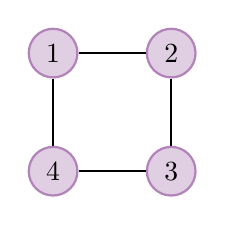
\begin{tikzpicture}
        \node (n4) at (0,0) [circle,draw=thupurple!50,fill=thupurple!20,thick] {4};
        \node (n1) at (0,1.5cm) [circle,draw=thupurple!50,fill=thupurple!20,thick] {1};
        \node (n3) at (1.5cm,0) [circle,draw=thupurple!50,fill=thupurple!20,thick] {3};
        \node (n2) at (1.5cm,1.5cm) [circle,draw=thupurple!50,fill=thupurple!20,thick] {2};
        \draw [semithick] (n1)--(n2)--(n3)--(n4)--(n1);
      \end{tikzpicture}
    \end{center}
    \begin{itemize}
    \item $a_{ii} = a_{ij} = 1/3$, for $j \in \mathcal N(i)$.
    \item We choose $\varphi = 0.9$.
    \end{itemize}
  \end{frame}

  \begin{frame}{Numerical Example: Convergence Result}
    \begin{figure}[ht]
      \begin{center}
        \setlength{\figureheight}{5cm}
        \setlength{\figurewidth}{6cm}
        \inputtikz{convergence}
      \end{center}
    \end{figure}
  \end{frame}

  \begin{frame}{Numerical Example:Estimation Performance}
    \begin{figure}[ht]
      \begin{center}
        \setlength{\figureheight}{5cm}
        \setlength{\figurewidth}{6cm}
        \inputtikz{variance}
      \end{center}
      \label{fig:variance}
    \end{figure}
  \end{frame}

  % \section{Conclusion}
  % \begin{frame}{Conclusion}
  %   \begin{itemize}
  %   \item We propose a privacy preserving average consensus algorithm.
  %   \item We compute the exact mean square convergence rate of the proposed algorithm.
  %   \item We derive the asymptotic estimation performance.
  %   \item We provide a topological necessary and sufficient condition, under which the privacy of an agent is breached. 
  %   \item We prove that our algorithm achieves minimum privacy breach, under the non-collaborating assumption.
  %   \item We prove that our consensus algorithm is differentially private given that $P_{ii}\neq 0$. 
  %   \end{itemize}
  %   
  % \end{frame}

  \section{Conclusion}

  % \begin{frame}{CPS Architecture}
  %   \begin{center}
  %     \begin{tikzpicture}[>=latex]
  %       \draw [draw=caltechcolor!50,fill=caltechcolor!20,thick] (-4,-0.5) rectangle (4,0.5);
  %       \node at (0,0) {Physical System};
  %       \draw [draw=blue!50,fill=blue!20,thick] (-4,1.5) rectangle (4,2.5);
  %       \node at (0,2) {Cyber Infrastructure};
  %       \draw [draw=red!50,fill=red!20,thick] (-4,3.5) rectangle (4,4.5);
  %       \node at (0,4) {Decision Making and Control};
  %       \node [anchor=west] at (2,3) {Raw Data};
  %       \node [anchor=east] at (-2,3) {Control};
  %       \draw [thick,->] (-2,3.5)--(-2,2.5);
  %       \draw [thick,->] (-2,1.5)--(-2,0.5);
  %       \draw [thick,<-] (2,3.5)--(2,2.5);
  %       \draw [thick,<-] (2,1.5)--(2,0.5);
  %     \end{tikzpicture}
  %   \end{center}
  % \end{frame}
  % 
  % \begin{frame}{A Secure CPS Architecture}
  %   \begin{center}
  %     \begin{tikzpicture}[>=latex]
  %       \draw [draw=caltechcolor!50,fill=caltechcolor!20,thick] (-4,-0.5) rectangle (4,0.5);
  %       \node at (0,0) {Physical System};
  %       \draw [draw=blue!50,fill=blue!20,thick] (-4,1.5) rectangle (4,2.5);
  %       \node at (0,2) {Cyber Infrastructure};
  %       \draw [draw=green!50,fill=green!20,thick] (-4,3.5) rectangle (4,4.5);
  %       \node at (0,4) {Security Layer};
  %       \draw [draw=red!50,fill=red!20,thick] (-4,5.5) rectangle (4,6.5);
  %       \node at (0,6) {Decision Making and Control};
  %       \node [anchor=west] at (2,3) {Raw Data};
  %       \node [anchor=west] at (2,5) {Secured Data};
  %       \node [anchor=east] at (-2,3) {Modified Control};
  %       \node [anchor=east] at (-2,5) {Control};
  %       \draw [thick,->] (-2,5.5)--(-2,4.5);
  %       \draw [thick,->] (-2,3.5)--(-2,2.5);
  %       \draw [thick,->] (-2,1.5)--(-2,0.5);
  %       \draw [thick,<-] (2,5.5)--(2,4.5);
  %       \draw [thick,<-] (2,3.5)--(2,2.5);
  %       \draw [thick,<-] (2,1.5)--(2,0.5);
  %     \end{tikzpicture}
  %   \end{center}
  % \end{frame}

  \begin{frame}{Conclusion}
    \begin{itemize}
    \item We consider the impact of replay attacks on a steady state control system and propose watermarking scheme to actively detect the presence of replay attack. For systems whose parameters are unknown, we design learning based mechanism to identify the parameters and design the watermarking signals simultaneously.
      \item We design an algorithm to achieve exact average consensus, while protecting the privacy of the initial state of each agent. We further prove that the proposed algorithm achieves minimum privacy breach.
    \end{itemize}
  \end{frame}

  \begin{frame}[standout]
    Thank you!
  \end{frame}

\end{document}

%%% Local Variables: 
%%% coding: utf-8
%%% mode: latex
%%% TeX-engine: xetex
%%% End: 